\documentclass[11pt]{article}
\usepackage[margin=0.7in]{geometry}
\usepackage[T1]{fontenc}
\usepackage{lmodern,graphicx,longtable,array,amsmath,amssymb,url,hyperref}
\hypersetup{hidelinks}
\setlength{\parindent}{0pt}\setlength{\parskip}{7pt}
\begin{document}
\raggedright
{\LARGE Published genus-2 law: independent scope review}\par
Review ID: published-law-scope-20261030. Task T-930. 30 October 2026.

\textbf{Scope.} Static source-to-claim inspection and retained verification evidence. No fresh compilation, Magma execution, census, solver, replay or benchmark. This packet records obligations and evidence boundaries; it supplies no new cost ratio or universal correctness theorem. The original full research objective remains incomplete.

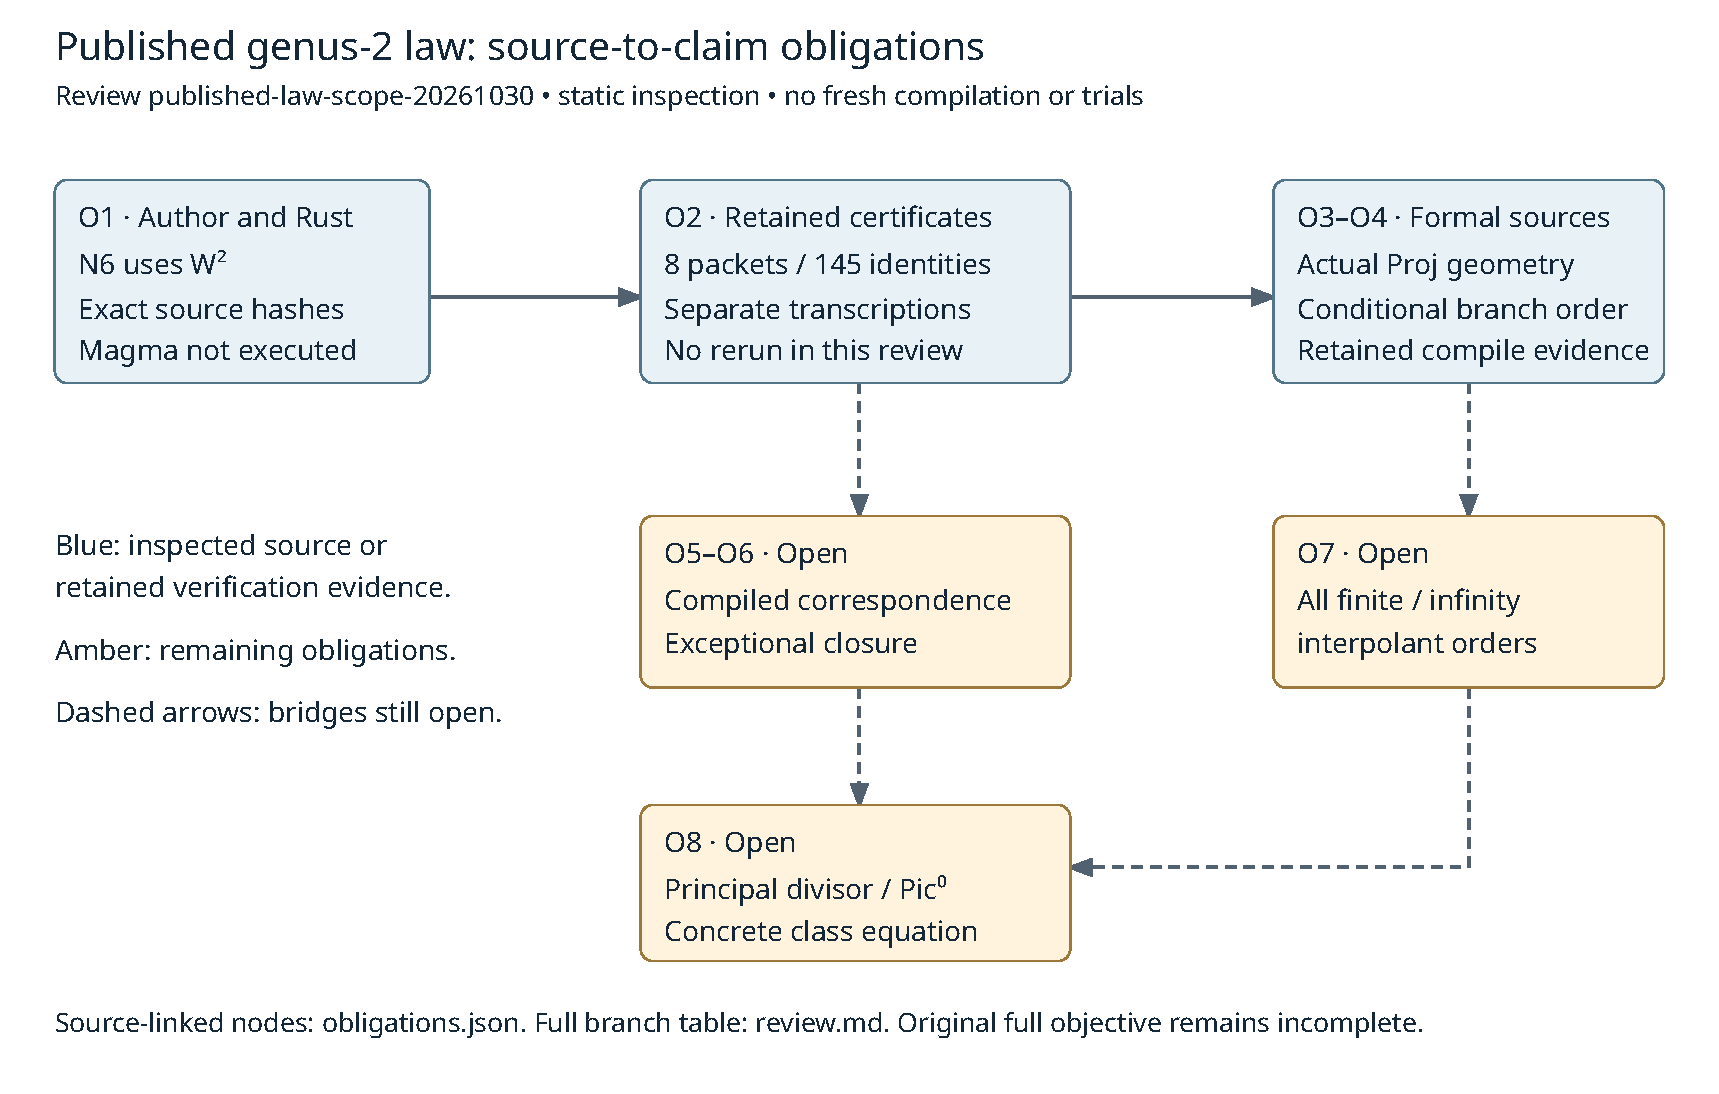
\includegraphics[width=\linewidth]{obligations-figure.pdf}

\textbf{Reading the diagram.} Blue boxes identify inspected source or previously retained evidence, not freshly rerun validation. Amber boxes identify open obligations. Solid arrows organize the evidence chain; they do not assert that a certificate alone proves the next theorem. Dashed arrows mark unresolved proof bridges. Node source paths and statuses are retained in \texttt{obligations.json}; the full branch table is in the unchanged \texttt{review.md}.

\textbf{Additive correction, 2026-10-30.} Later formal sources already include actual weighted-Proj smoothness, the glued-model-to-Proj isomorphism, and a conditional actual-quintic rational-branch order theorem. Older checklist descriptions that these bridges are wholly missing are stale. Historical files remain unchanged. Compiled semantics and global divisor-class obligations remain open.
\newpage
{\Large Branch obligations and input model}\par
The intended model is a smooth odd-characteristic curve
$y^2=x^5+a_3x^3+a_2x^2+a_1x+a_0$, valid reduced Mumford divisors, nonzero weights and consistent field/curve parameters. Runtime entry points do not check every mathematical hypothesis.

Degree one represents $x=X/Z^2$, $y=Y/(Z^5W)$. Degree two represents
$u=x^2+(Q/Z^2)x+R/Z^4$, $v=(S/(Z^3W))x+T/(Z^5W)$.

\small
\begin{longtable}{p{0.18\linewidth}p{0.36\linewidth}p{0.38\linewidth}}
\textbf{Branch} & \textbf{Observed source behavior} & \textbf{Remaining universal obligation}\\\hline
1+1 & Inverse first; then doubling; otherwise distinct-x output. & Nonzero weights, tangency/chord multiplicities and infinity.\\
Generic 1+2 & Nonzero K gives degree two; 16 retained identities. & Runtime-polynomial link, residual sign and principal divisor.\\
Exceptional 1+2 & Cancellation, tripling, or double-plus-other; 12 exception and 16 triple identities. & Exclude mismatch/secondary failure; repeated-root multiplicities.\\
Same-u 2+2 & Inverse, equal-v double, or mixed extracted-point double; mixed 7 identities. & Valid-input zero-slope exclusion and canceled components.\\
Doubling & B=0 subcases; otherwise C=0 degree drop or degree two; 30 identities. & Closure and valid nonzero output weights on every subcase.\\
Shared-support & Cancel shared point or double and add remaining points; 27 identities. & None unreachability, including intermediate degree drops.\\
Coprime drop & B nonzero, C zero gives degree one; 18 identities. & Exhaustive parametrization and residual/infinity multiplicity.\\
Coprime common & B,C nonzero gives degree two; 19 identities. & Compiled numerator correspondence and all-place divisor equation.\\\hline
\end{longtable}
\normalsize
The eight certificate outputs total 145 polynomial identities. They are separately transcribed calculations, not a mechanical proof of every compiled statement. The public projective dispatcher uses \texttt{expect}; an unreachable-None proof is a completeness obligation, not a fallback to Cantor arithmetic.

\textbf{W squared.} The exact pinned author \texttt{DBL2} defines $WW1=W1^2$ and uses it in N6. Production Rust also selects $W^2$. The $W^1$ variant is a deliberate mutation test, not a demonstrated defect in the published source.

\textbf{Inversions.} Inspected formula branches have no explicit inversion. Nonidentity normalization calls inverse twice (Z and W); identity calls none. This does not establish an inversion-free collector or end-to-end pipeline.
\newpage
{\Large Formal scope, retained context and references}\par
\texttt{WeightedProjSmoothFinal.smooth} and \texttt{WeightedProjCrossInjective.gluedToProj\_isIso} address actual projective geometry. \texttt{WeightedProjInfinityDVR} establishes local infinity facts, including order two for Z; it does not yet identify the interpolation function's complete pole divisor.

\texttt{WeightedProjSourceBranchActualQuintic} proves order one in an actual projective branch stalk for the proof-side common-2+2 expression under valid input congruences, nonzero determinant, rational branch and support-root hypotheses. Its separable corollary supplies simple-root geometry. It is not a theorem about every compiled Rust branch.

\texttt{RuntimeSemantics.residual\_represents\_input} assumes a principal-divisor/class interface and the required principal-divisor premise. It gives the abstract class consequence; constructing the concrete interface and premise remains necessary. Saved records report Lean checks without \texttt{sorryAx}; this review inspected declarations and retained records, without compiling them anew.

\textbf{Retained finite context, not new measurements.} The historical projective-law report records two collector arms, each over 1,260 frozen targets with paired source-rho controls. Its wrapper normalizes every addition; retained state normalizes at relation boundaries. This review does not recompute its counts or prices. Finite successes do not prove universal completeness. The public-source parity report records 34,704 translated-author/Rust comparisons and 34,704 Rust/Cantor comparisons over two finite fields. That was restricted translation of source, not actual Magma execution.

\textbf{Next proof work.} Bind actual runtime expressions and predicates to the existing polynomials; prove exceptional closure and returned-weight nonvanishing; complete interpolant orders at nonbranch points, repeated supports and infinity; construct the global principal divisor and concrete Pic$^0$ equality. Extend across every branch and handle nonsplit places if the theorem quantifies over arbitrary fields.

\textbf{References and provenance.} Paths are repository-relative; exact inspected file hashes are in \texttt{source-hashes.sha256}. The original review is preserved byte-for-byte.
\par Study root:\par \texttt{research/projective\_law\_followup\_20261022}.\par
Relative references below use that root. Full paths and hashes are in the JSON and hash manifest.
\begin{itemize}
\item \texttt{src/bin/projective\_law\_gate.rs}; \texttt{formal/RuntimeSemantics.lean}.
\item \texttt{PROOF\_AUDIT.md}; \texttt{formal/PROJECTIVE\_BRANCH\_ZERO\_ORDER.md}.\par Eight \texttt{results/symbolic-*.json} records.
\item \texttt{REPORT.md}; \texttt{public\_source\_parity/README.md}.\par \texttt{n6-homogeneity/source-correction/README.md}.
\item Pinned author repository: \url{https://github.com/ozbayelif/jac-on-jac}. \par Commit \texttt{ec98e115ed359c8b7facf559eb0d9f240703f6f5},\par file \texttt{jac-on-jac.m}. Downloaded bytes matched the retained SHA-256; no author program was executed.
\end{itemize}
\end{document}
